\documentclass[11pt,a4paper]{article}
\usepackage[a4paper]{geometry}
\usepackage[utf8]{inputenc}
\usepackage[english]{babel}
\usepackage{lipsum}
\usepackage{eurosym}
\usepackage{rotating}

\usepackage{amsmath, amssymb, amsfonts, amsthm, mathtools}
% mathtools for: Aboxed (put box on last equation in align environment)
\usepackage{microtype} %improves the spacing between words and letters

\usepackage{lipsum}
\usepackage{threeparttable}
\usepackage{tabularx}
\usepackage{multirow}
\usepackage{booktabs}
\newcommand{\tabitem}{~~\llap{\textbullet}~~}
\usepackage{graphicx}
\graphicspath{ {./figures/} {./eps/}}
\usepackage{epsfig}
\usepackage{epstopdf}
\usepackage{verbatim}
\usepackage{textcomp}
\usepackage{tikz}
\usetikzlibrary{shapes,arrows}

\geometry{vmargin={2cm, 2cm}}

%%%%%%%%%%%%%%%%%%%%%%%%%%%%%%%%%%%%%%%%%%%%%%%%%%
%% COLOR DEFINITIONS
%%%%%%%%%%%%%%%%%%%%%%%%%%%%%%%%%%%%%%%%%%%%%%%%%%
 % Enabling mixing colors and color's call by 'svgnames'
%%%%%%%%%%%%%%%%%%%%%%%%%%%%%%%%%%%%%%%%%%%%%%%%%%
\definecolor{MyColor1}{HTML}{CC0000} %mix personal color
\newcommand{\textb}{\color{Black} \usefont{OT1}{lmss}{m}{n}}
\newcommand{\blue}{\color{MyColor1} \usefont{OT1}{lmss}{m}{n}}
\newcommand{\blueb}{\color{MyColor1} \usefont{OT1}{lmss}{b}{n}}
\newcommand{\red}{\color{LightCoral} \usefont{OT1}{lmss}{m}{n}}
\newcommand{\green}{\color{Turquoise} \usefont{OT1}{lmss}{m}{n}}
%%%%%%%%%%%%%%%%%%%%%%%%%%%%%%%%%%%%%%%%%%%%%%%%%%

%%%%%%%%%%%%%%%%%%%%%%%%%%%%%%%%%%%%%%%%%%%%%%%%%%
%% Scala coloring settings
%%%%%%%%%%%%%%%%%%%%%%%%%%%%%%%%%%%%%%%%%%%%%%%%%%
% "define" Scala
\usepackage{listings}
\usepackage[framed, numbered]{matlab-prettifier}
\usepackage{xcolor}
\lstset{escapeinside={<@}{@>}}

\definecolor{dkgreen}{rgb}{0,0.6,0}
\definecolor{gray}{rgb}{0.5,0.5,0.5}
\definecolor{mauve}{rgb}{0.58,0,0.82}
\definecolor{cri1}{HTML}{2D85FF}
\definecolor{cri2}{HTML}{FF006E}
\definecolor{cri3}{HTML}{0008FF}
\definecolor{cri4}{HTML}{00A9FF}
\definecolor{cri5}{HTML}{55CF7D}
\definecolor{cri6}{HTML}{FFAF1C}

\lstdefinestyle{myScalastyle}{
  frame=tb,
  language=scala,
  aboveskip=3mm,
  belowskip=3mm,
  showstringspaces=false,
  columns=flexible,
  basicstyle={\small\ttfamily},
  numbers=none,
  numberstyle=\tiny\color{gray},
  keywordstyle=\color{blue},
  commentstyle=\color{dkgreen},
  stringstyle=\color{mauve},
  frame=single,
  breaklines=true,
  breakatwhitespace=true,
  tabsize=3,
}

\lstdefinestyle{myBashstyle}{
  frame=tb,
  language=bash,
  aboveskip=3mm,
  belowskip=3mm,
  showstringspaces=false,
  columns=flexible,
  basicstyle={\small\ttfamily},
  numbers=none,
  numberstyle=\tiny\color{gray},
  keywordstyle=\color{cri2},
  commentstyle=\color{cri1},
  stringstyle=\color{cri6},
  % <@\textcolor{cri5}{'Ziggy is running the Recommender...'}@>
  % <@\textcolor{cri5}{'Adding dataset to Hadoop...'}@>
  % <@\textcolor{cri5}{'Creating directory...'}@>
  % <@\textcolor{cri5}{'Adding user_artist_data.txt...'}@>
  % <@\textcolor{cri5}{'Adding artist_data.txt...'}@>
  % <@\textcolor{cri5}{'Adding artist_alias.txt...'}@>
  frame=single,
  breaklines=true,
  breakatwhitespace=true,
  tabsize=3,
}
%%%%%%%%%%%%%%%%%%%%%%%%%%%%%%%%%%%%%%%%%%%%%%%%%%
%% FONTS AND COLORS
%%%%%%%%%%%%%%%%%%%%%%%%%%%%%%%%%%%%%%%%%%%%%%%%%%
%		SECTIONS
%%%%%%%%%%%%%%%%%%%%%%%%%%%%%%%%%%%%%%%%%%%%%%%%%%
\usepackage{titlesec}
\usepackage{sectsty}
%%%%%%%%%%%%%%%%%%%%%%%%
%set section/subsections HEADINGS font and color
\sectionfont{\color{MyColor1}}  % sets colour of sections
\subsectionfont{\color{MyColor1}}  % sets colour of sections

%set section enumerator to arabic number (see footnotes markings alternatives)
\renewcommand\thesection{Exercise \arabic{section}} %define sections numbering
\renewcommand\thesubsection{\thesection.\arabic{subsection}} %subsec.num.

%define new section style
\newcommand{\mysection}{
\titleformat{\section} [runin] {\usefont{OT1}{lmss}{b}{n}\color{MyColor1}}
{\thesection} {3pt} {} }

%%%%%%%%%%%%%%%%%%%%%%%%%%%%%%%%%%%%%%%%%%%%%%%%%%
%		CAPTIONS
%%%%%%%%%%%%%%%%%%%%%%%%%%%%%%%%%%%%%%%%%%%%%%%%%%
\usepackage{caption}
\usepackage{subcaption}
%%%%%%%%%%%%%%%%%%%%%%%%
\captionsetup[figure]{labelfont={color=MyColor1}}

%%%%%%%%%%%%%%%%%%%%%%%%%%%%%%%%%%%%%%%%%%%%%%%%%%
%		!!!EQUATION (ARRAY) --> USING ALIGN INSTEAD
%%%%%%%%%%%%%%%%%%%%%%%%%%%%%%%%%%%%%%%%%%%%%%%%%%
%using amsmath package to redefine eq. numeration (1.1, 1.2, ...)
%%%%%%%%%%%%%%%%%%%%%%%%
\renewcommand{\theequation}{\arabic{equation}}

%set box background to grey in align environment
\usepackage{etoolbox}% http://ctan.org/pkg/etoolbox
\makeatletter
\patchcmd{\@Aboxed}{\boxed{#1#2}}{\colorbox{black!15}{$#1#2$}}{}{}%
\patchcmd{\@boxed}{\boxed{#1#2}}{\colorbox{black!15}{$#1#2$}}{}{}%
\makeatother
%%%%%%%%%%%%%%%%%%%%%%%%%%%%%%%%%%%%%%%%%%%%%%%%%%

\newcommand{\DP}[1]{\textcolor{blue}{\textbf{(DP says: #1)}}}

\makeatletter
\let\reftagform@=\tagform@
\def\tagform@#1{\maketag@@@{(\ignorespaces\textcolor{red}{#1}\unskip\@@italiccorr)}}
\renewcommand{\eqref}[1]{\textup{\reftagform@{\ref{#1}}}}
\makeatother
\usepackage[hidelinks]{hyperref}

%% LISTS CONFIGURATION %%
\usepackage{enumitem}
\setlist[enumerate,1]{start=0}
\renewcommand{\labelenumii}{\theenumii}
\renewcommand{\theenumii}{\theenumi.\arabic{enumii}.}

\usepackage[acronym]{glossaries}
\newacronym{ci}{CI}{Confidence Interval}
\newacronym{pi}{PI}{Prediction Interval}

%%%%%%%%%%%%%%%%%%%%%%%%%%%%%%%%%%%%%%%%%%%%%%%%%%
%% PREPARE TITLE
%%%%%%%%%%%%%%%%%%%%%%%%%%%%%%%%%%%%%%%%%%%%%%%%%%
\title{\blue Network analysis and simulation\\ Homework 1}
\author{Davide Peron}
\date{}
%%%%%%%%%%%%%%%%%%%%%%%%%%%%%%%%%%%%%%%%%%%%%%%%%%

\begin{document}
\maketitle
\section{}
In the first exercise two datasets are given and on those, a bunch of figures have been plotted, in which the data are showed and different measures of confidence are calculated on them.

In the follow the said figures are reported.

\begin{figure}[ht]
	\centering
	\begin{minipage}{0.45\textwidth}
		\centering
		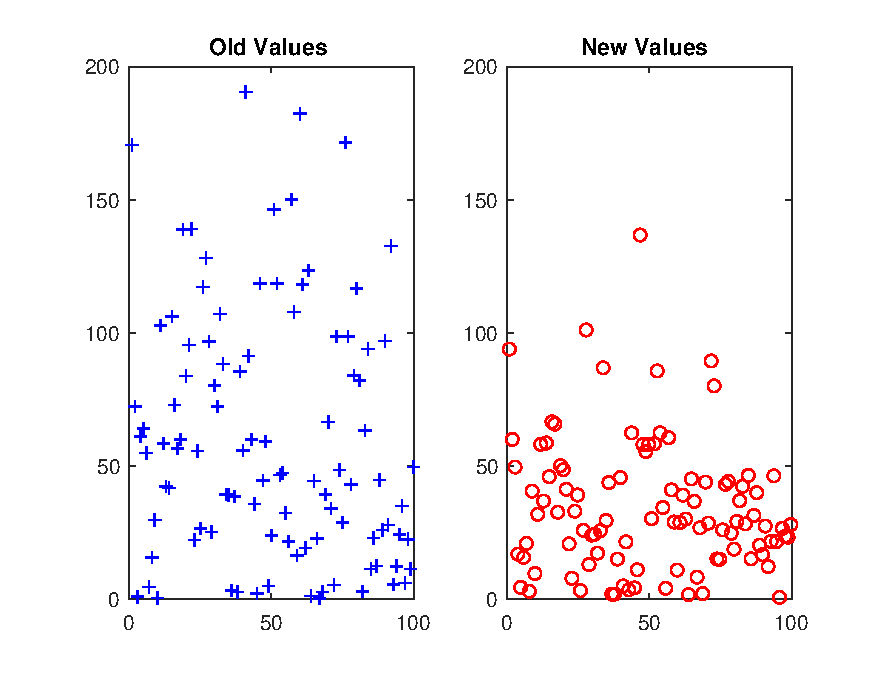
\includegraphics[width=\textwidth]{ex1fig2_1a}
		\caption{Plot of the data}
		\label{fig:data_exec}
	\end{minipage}
	\begin{minipage}{0.45\textwidth}
		\centering
		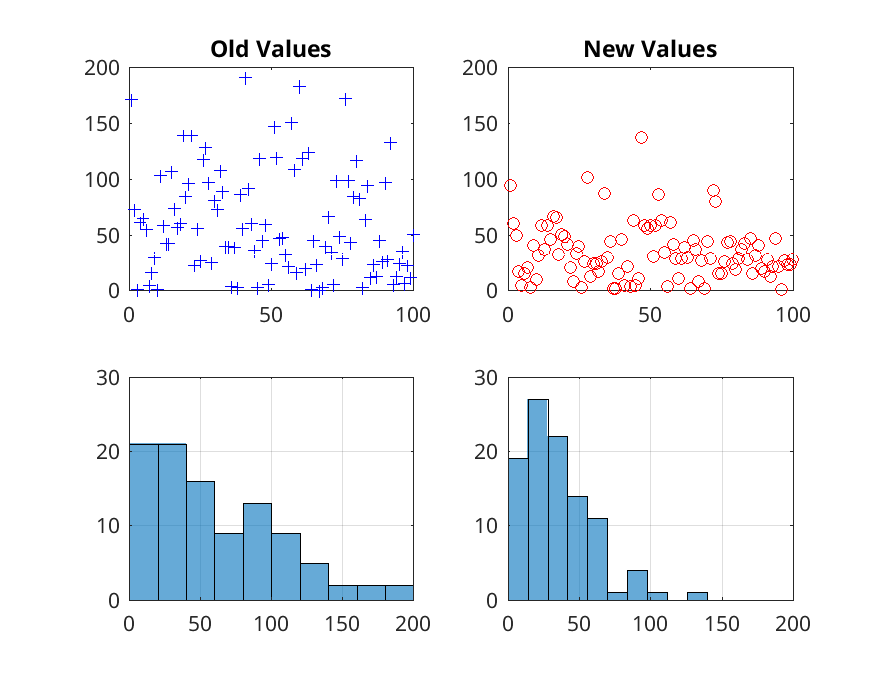
\includegraphics[width=\textwidth]{ex1fig2_1}
		\caption{Data plotted also in histograms divided in 10 bins (Figure 2.1)}
		\label{fig:data_exec_hist}
	\end{minipage}
\end{figure}

\begin{figure}[ht]
	\centering
	\begin{minipage}{0.45\textwidth}
		\centering
		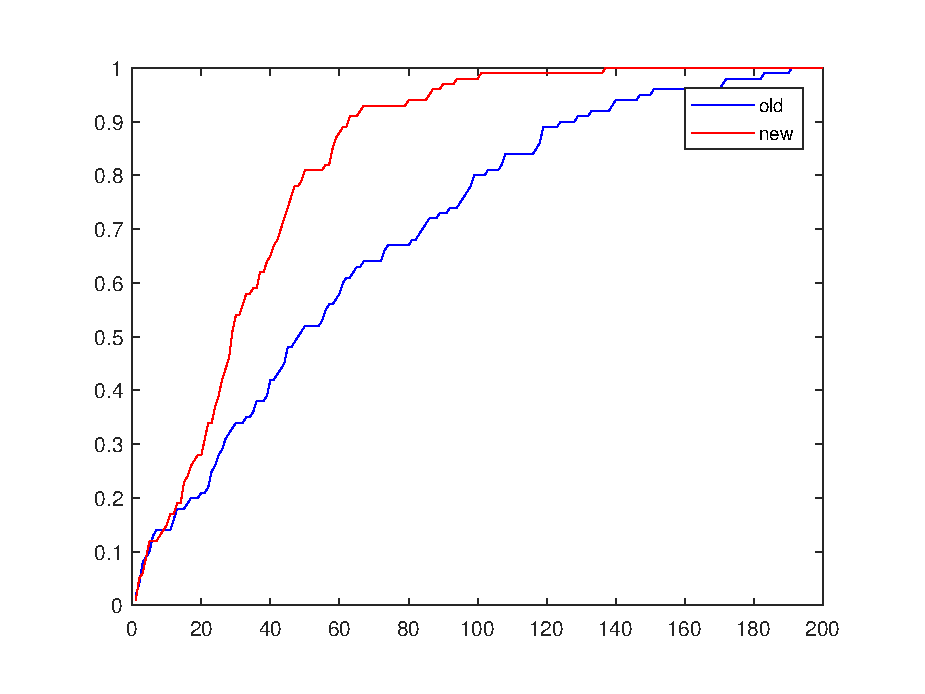
\includegraphics[width=\textwidth]{ex1fig2_2}
		\caption{Empirical distribution function of the data (Figure 2.2) }
		\label{fig:edf_exec}
	\end{minipage}
	\begin{minipage}{0.45\textwidth}
		\centering
		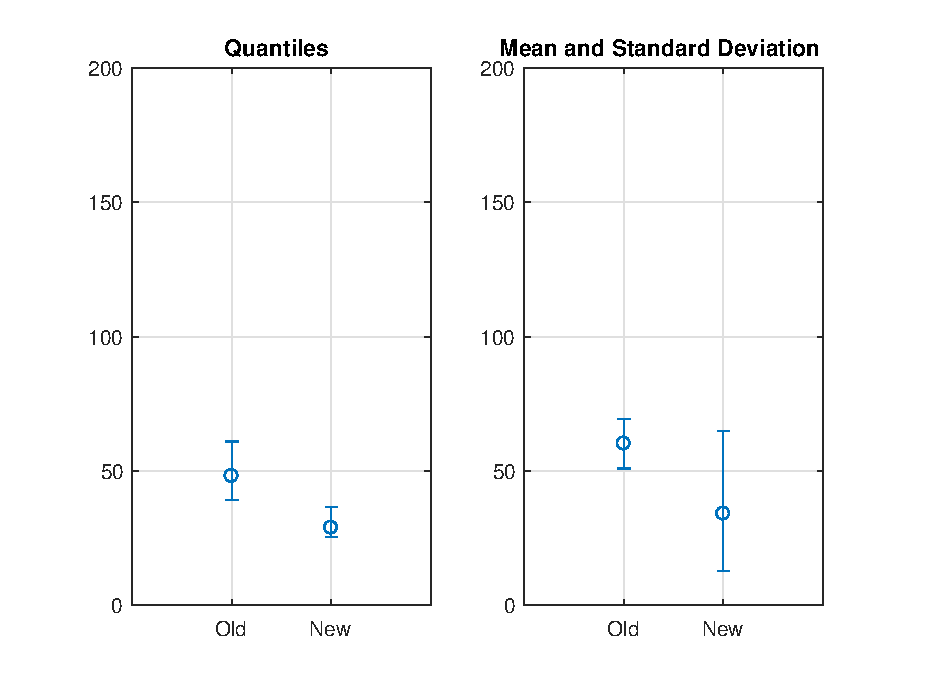
\includegraphics[width=\textwidth]{ex1fig2_3}
		\caption{Box Plots of the data with \gls{ci} for median and mean (Figure 2.3)}
		\label{fig:box_plots_exec}
	\end{minipage}
\end{figure}

\begin{figure}[ht]
	\centering
	\begin{minipage}{0.45\textwidth}
		\centering
		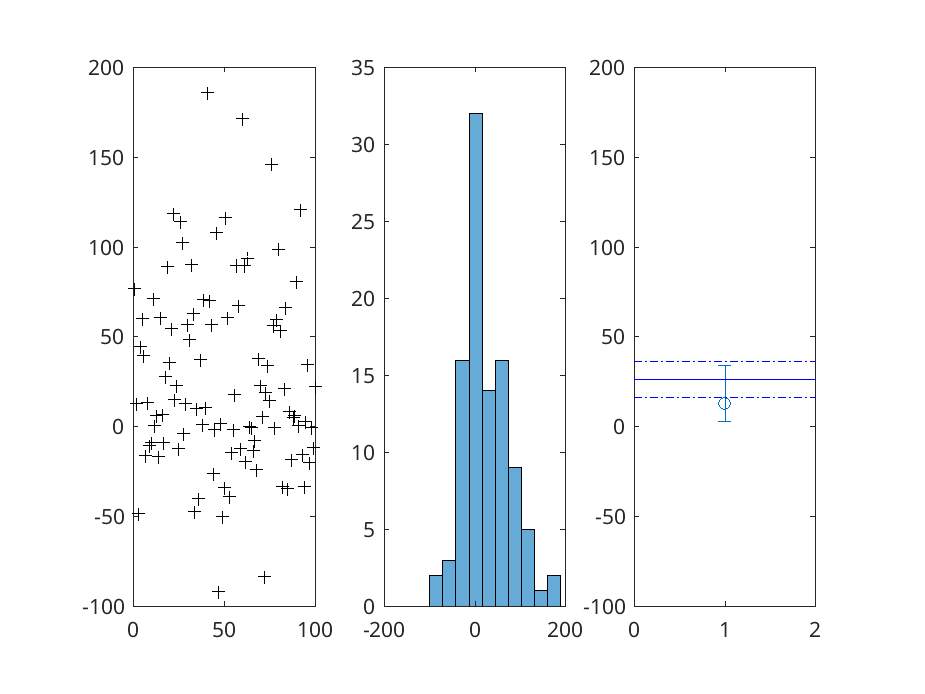
\includegraphics[width=\textwidth]{ex1fig2_7}
		\caption{Difference between old and new data (Figure 2.7) }
		\label{fig:diff_exec}
	\end{minipage}
	\begin{minipage}{0.45\textwidth}
		\centering
		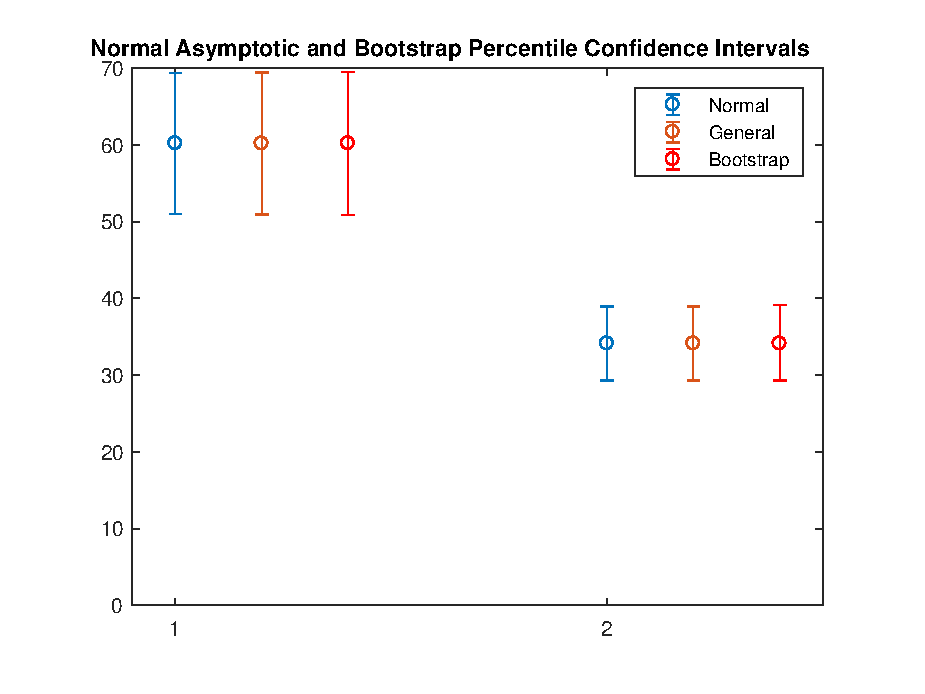
\includegraphics[width=\textwidth]{ex1fig2_8}
		\caption{Normal Asymptotic and Bootstrap Percentile Confidence Intervals (Figure 2.8)}
		\label{fig:figure2_8}
	\end{minipage}
\end{figure}

\begin{figure}[ht]
	\centering
	\begin{minipage}{0.45\textwidth}
		\centering
		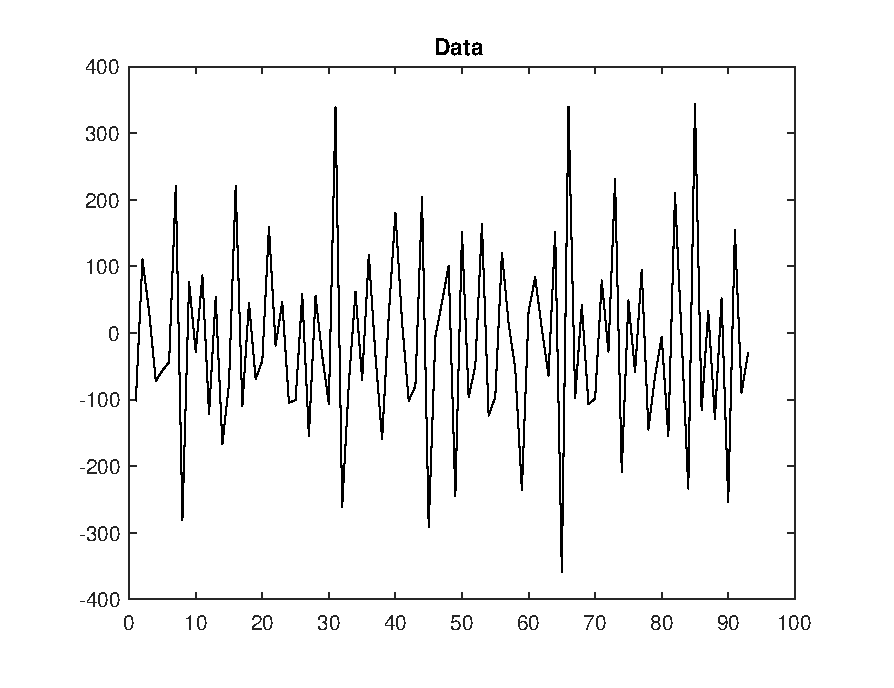
\includegraphics[width=\textwidth]{ex1fig2_10a}
		\caption{(Figure 2.10a)}
		\label{fig:figure2_10a}
	\end{minipage}
	\begin{minipage}{0.45\textwidth}
		\centering
		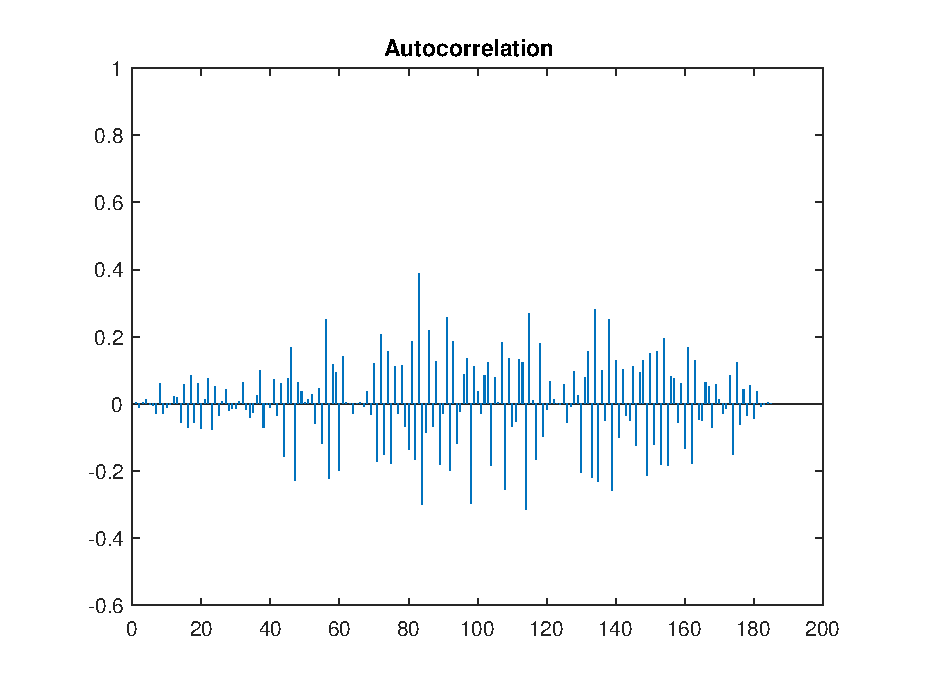
\includegraphics[width=\textwidth]{ex1fig2_10c}
		\caption{Autocorrelation of the plot in \autoref{fig:figure2_10a}(Figure 2.10c)}
		\label{fig:figure2_10c}
	\end{minipage}
\end{figure}

\begin{figure}[ht]
  \centering
  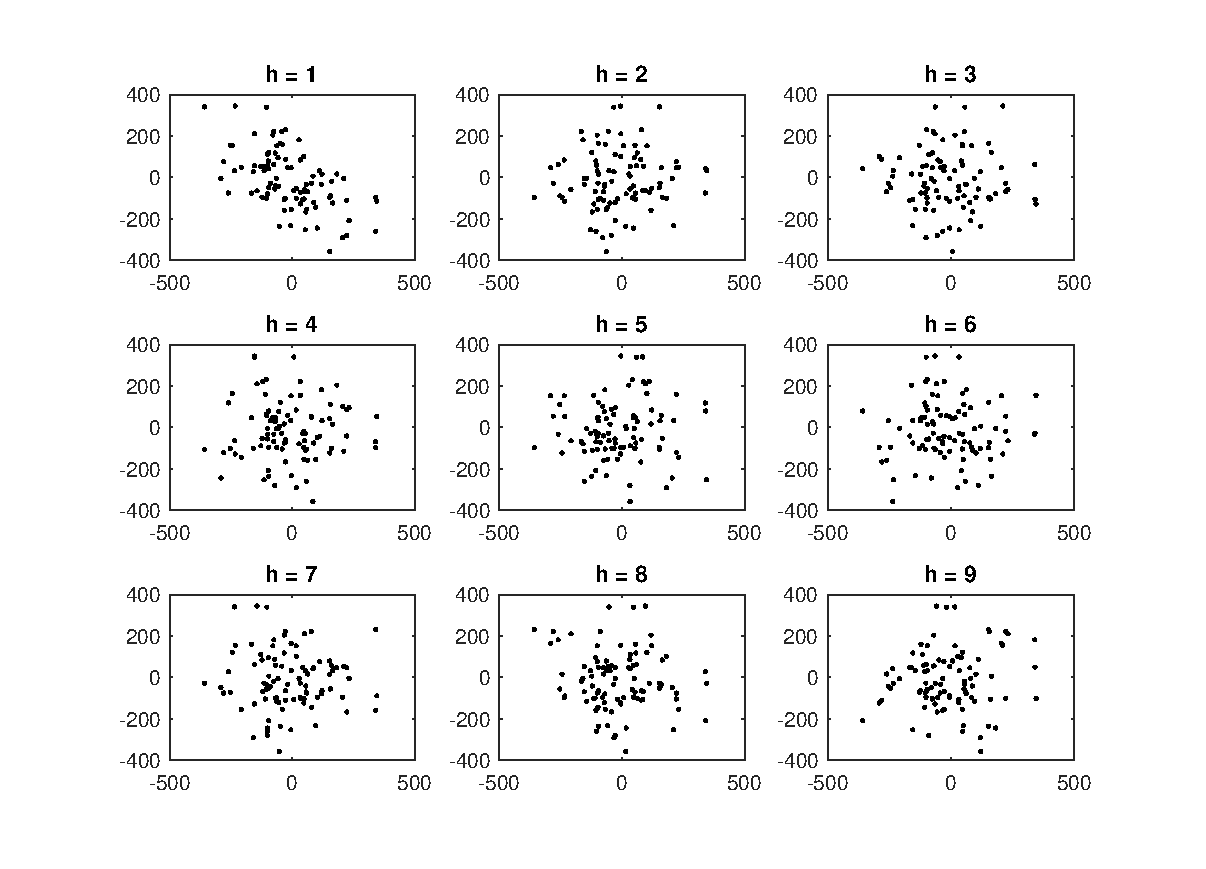
\includegraphics[width=0.9\textwidth]{ex1fig2_10d}
  \caption{Lag plots (Figure 2.10d)}
  \label{fig:lag_plot}
\end{figure}

\newpage
\section{}

Executing the script correspondent to the second exercise, we found that in 56 experiments the \gls{ci} does not contain the true value of the mean.

In \autoref{fig:CI_48_2} and \autoref{fig:CI_10002} are reported the value of the sample mean and its \gls{ci} (with $\gamma=0.95$) for each experiment, sorted based on the lower extreme of the \gls{ci} and using a different number of random variables in each experiment.
In both cases, the sample mean is distributed around the true mean (that for this Uniform Distribution is $0.5$).

Note how, increasing the number of random variables per experiment, the mean width of the \gls{ci} get lower.

\begin{figure}[ht]
	\centering
	\begin{minipage}{0.45\textwidth}
		\centering
		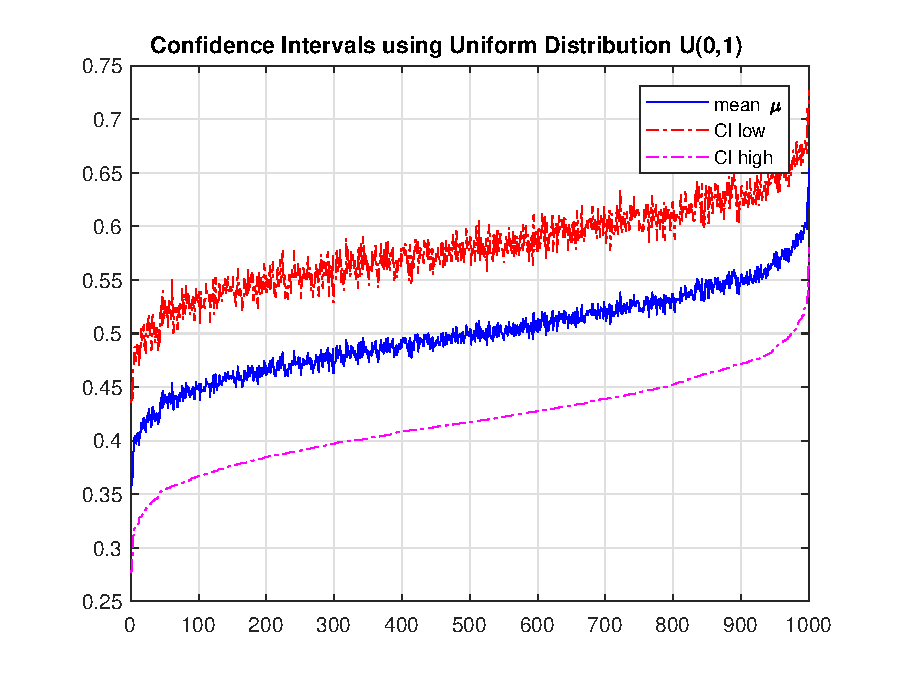
\includegraphics[width=\textwidth]{CI_48_2}
		\caption{Results of the experiment with $n=48$}
		\label{fig:CI_48_2}
	\end{minipage}
	\begin{minipage}{0.45\textwidth}
		\centering
		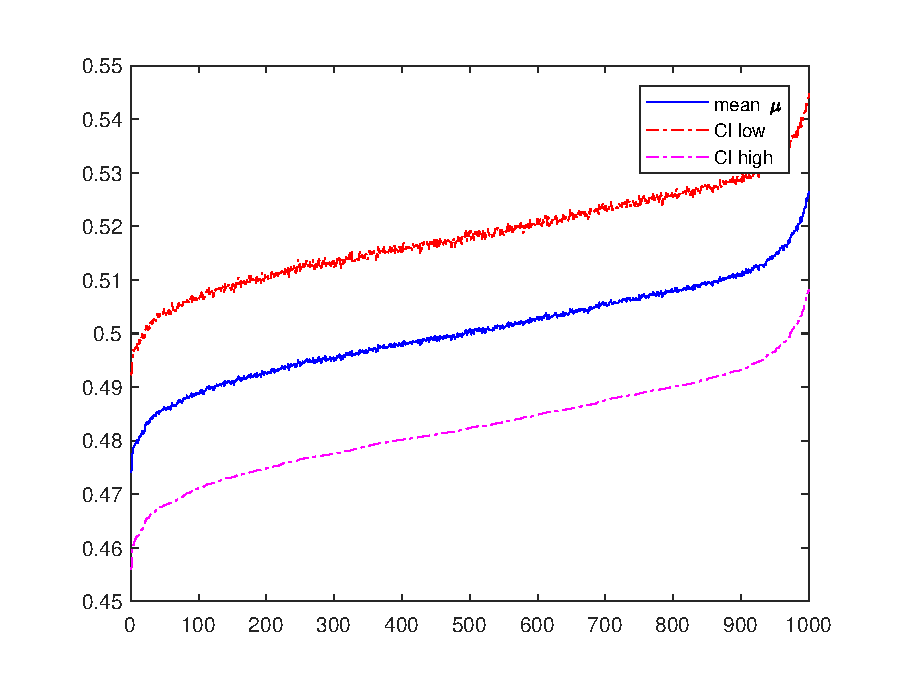
\includegraphics[width=\textwidth]{CI_10002}
		\caption{Results of the experiment with $n=1000$}
		\label{fig:CI_10002}
	\end{minipage}
\end{figure}

\section{}

To calculate $\mathbf{E}(U_{(j)})$ we have firstly to compute the probability that at least an order statistic $U_{(j)}$ falls in $[u, u+du]$, that is $P_{U_{(j)}}(u)$. Actually the probability that more than one element falls in this interval is negligigble since is an $O(du^2)$, so we can take in account only the probability that exactly one element falls in $[u, u+du]$.

This probability is given by the following expression:

\begin{equation}\label{eq:p(u)}
  \begin{split}
    P_{U_{(j)}}(u) = P\bigg[\text{$j-1$ order statistics are in $[0, u]$}\bigg] &\cdot P\bigg[\text{1 order statistic is in $[u, u+du]$}\bigg] \\&\cdot P\bigg[\text{$n-j$ order statistics are in $[u+du, 1]$}\bigg]
  \end{split}
\end{equation}

The probability that a realization of a random variable $\mathbf{U}(0,1)$ is in $[0, u]$ is $u$, we want $j-1$ realization over $n$ to be in this interval, so the resulting probability is:
$$
P\bigg[\text{$j-1$ order statistics are in $[0, u]$}\bigg] = \binom{n}{j-1}u^{j-1}
$$
Now we want the next order statistic to be in $[u, u+du]$, so we can choose from the remaining $n-j+1$ realization an element with probability $du$, that is:
$$ P\bigg[\text{1 order statistic is in $[u, u+du]$}\bigg] = (n-j+1)du$$
Finally, the last $n-j$ elements have to be in $[u+du,1]$, so:
$$ P\bigg[\text{$n-j$ order statistics are in $[u+du, 1]$}\bigg] = (1-u-du)^{n-j} $$
but since $du$ is very small by definition, we can ignore it rewriting this last equation as $(1-u)^{n-j}$.

Multiplying these three terms, as specified in \autoref{eq:p(u)}, the final probability is:
\begin{equation}
  \label{eq:pu_calculated}
  P_{U_{(j)}}(u) = \frac{n!}{(j-1)!(n-j)!}u^{j-1}\cdot du \cdot (1-u)^{n-j}
\end{equation}

The keypoint of the proof is to note that \autoref{eq:pu_calculated} is the PDF of a Beta distribution.
Indeed a general Beta distribution is defined as
\begin{equation}
  \label{eq:beta}
  f(x) = \frac{1}{\mathbf{B}(\alpha,\beta)}x^{\alpha-1}(1-x)^{\beta-1}
\end{equation}
where $\mathbf{B}(\alpha,\beta)$ is called \textit{Beta function} and is defined as
\begin{equation}
  \label{eq:beta_func}
  \mathbf{B}(\alpha,\beta) = \frac{(\alpha-1)!(\beta-1)!}{(\alpha+\beta-1)!}
\end{equation}

Given this definition, we can derive that $P_{U_{(j)}}(u)$ is distributed as a $Beta(j,n+1-j)$ and since the expected value of a \textit{Beta} distribution is defined as $\mathbf{E}[x] = \frac{\alpha}{\alpha+\beta}$, we conclude that
\begin{equation}
  \label{eq:ex_value}
  \mathbf{E}\bigg[U_{(j)}\bigg] = \frac{j}{n+1}
\end{equation}

\section{}

In \autoref{fig:ex4_accuracy} is plotted the accuracy of the sample mean versus the number of random variables in each experiment. This measure have been made based on the following formula:
\begin{equation}
  A_i = |\overline{x_i} - \overline{x}|
\end{equation}
where $A_i$ is the accuracy of the experiment $i$ and $x_i$ is the sample mean of the same experiment. As can be seen in the said figure, the error from the true value get lower as the number of random variables in each experiment increase, this happens since the higher is the number of random variables, the higher is the precision of the experiment.

In \autoref{fig:ex4_CI} is reported the variance of each experiment and the relative confidence interval computed using bootstrap method.
Finally, in \autoref{fig:PI_theory} and \autoref{fig:PI_bootstrap} are reported the prediction intervals at level $\gamma = 0.95$ using theory and using bootstrap.

\begin{figure}[ht]
	\centering
	\begin{minipage}{0.45\textwidth}
		\centering
		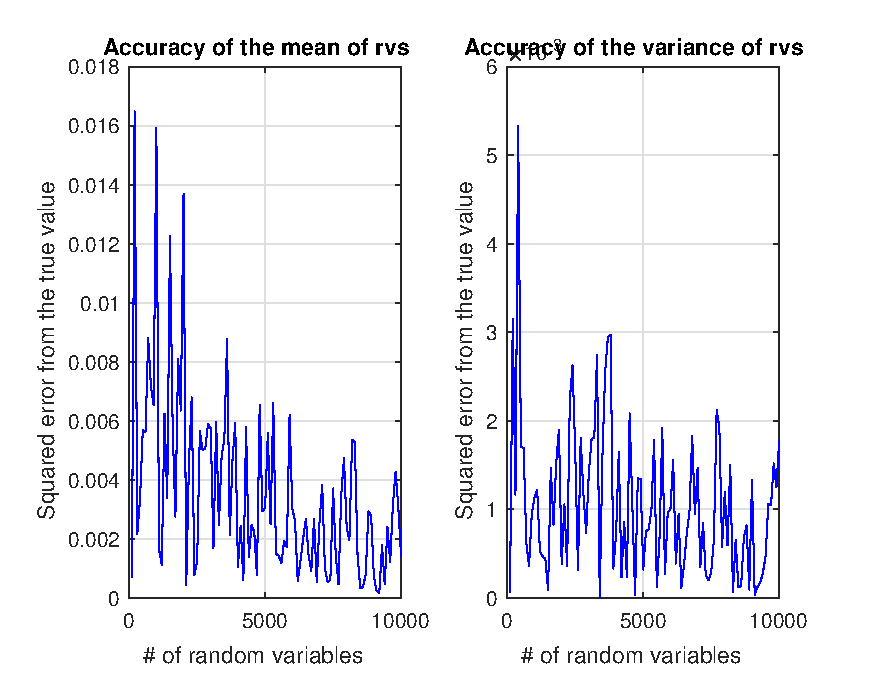
\includegraphics[width=\textwidth]{ex4_accuracy}
		\caption{Accuracy of the estimation versus $n$}
		\label{fig:ex4_accuracy}
	\end{minipage}
	\begin{minipage}{0.45\textwidth}
		\centering
		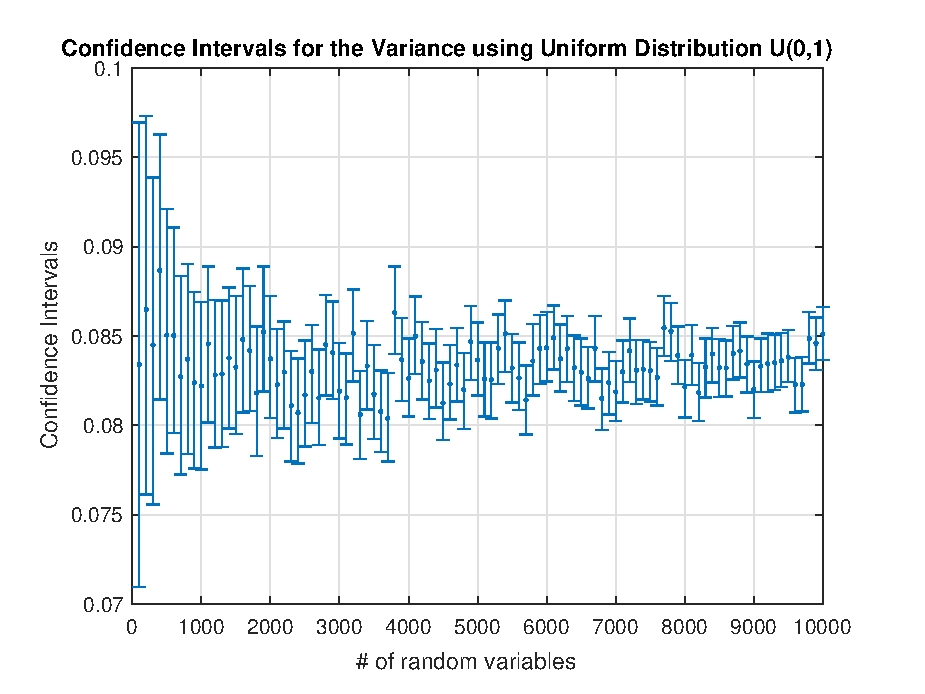
\includegraphics[width=\textwidth]{ex4_CI}
		\caption{Confidence intervals for the variance using rvs $U(0,1)$}
		\label{fig:ex4_CI}
	\end{minipage}
\end{figure}

\begin{figure}[ht]
	\centering
	\begin{minipage}{0.45\textwidth}
		\centering
		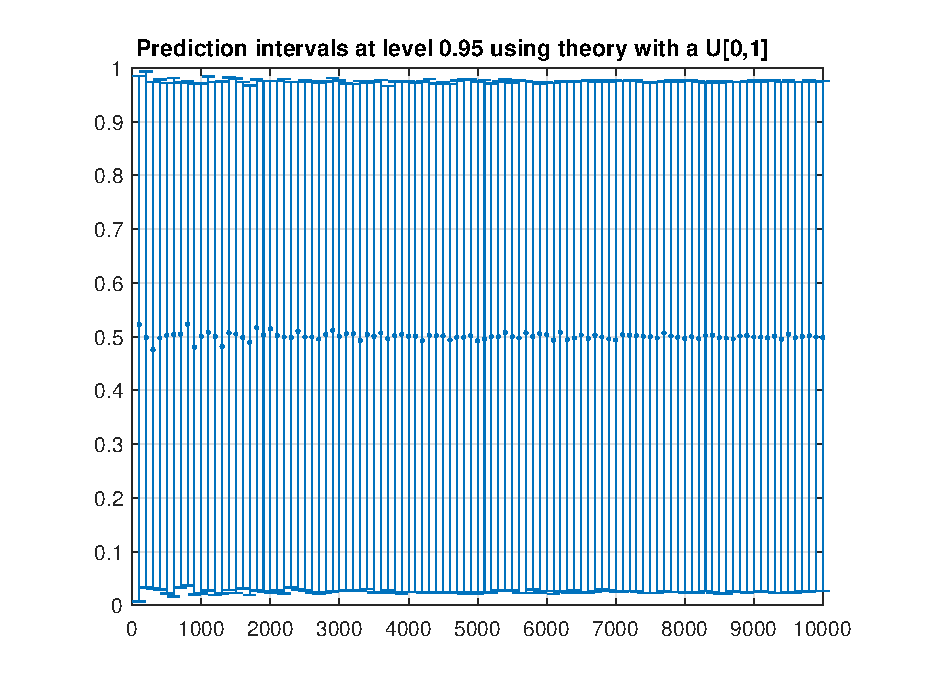
\includegraphics[width=\textwidth]{PI_theory}
		\caption{Prediction interval for a $U(0,1)$ at level $\gamma = 0.95$ using theory}
		\label{fig:PI_theory}
	\end{minipage}
	\begin{minipage}{0.45\textwidth}
		\centering
		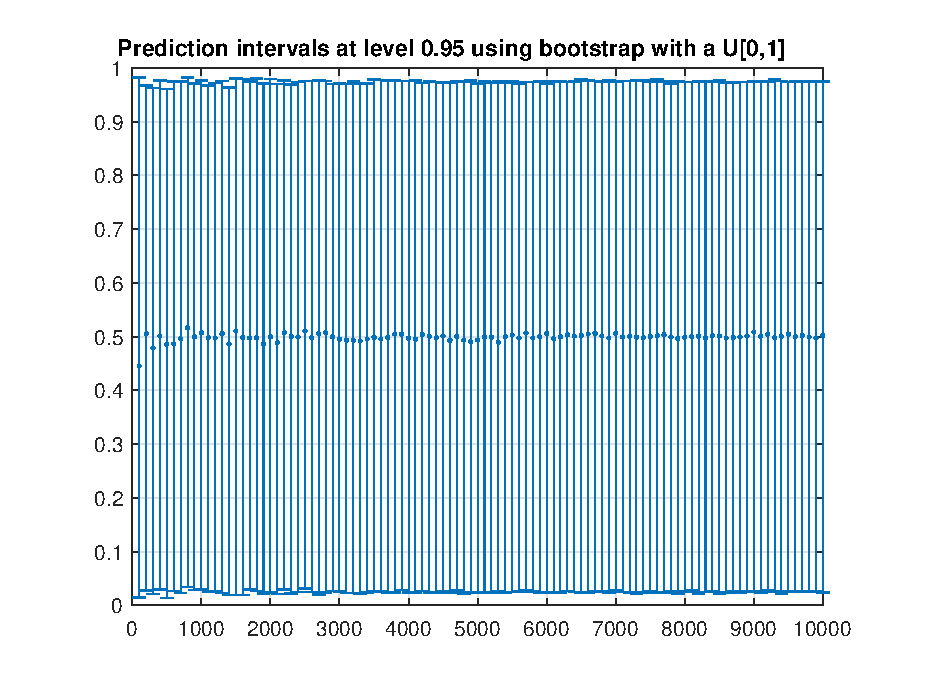
\includegraphics[width=\textwidth]{PI_bootstrap}
		\caption{Prediction interval for a $U(0,1)$ at level $\gamma = 0.95$ using bootstrap}
		\label{fig:PI_bootstrap}
	\end{minipage}
\end{figure}

\section{}

Redoing Exercise 2, the plots in \autoref{fig:ex2_48_N} and \autoref{fig:ex2_1000_N} have been obtained.
Note that the sample mean now is distributed around the new true value, that is $0$.

\begin{figure}[ht]
	\centering
	\begin{minipage}{0.45\textwidth}
		\centering
		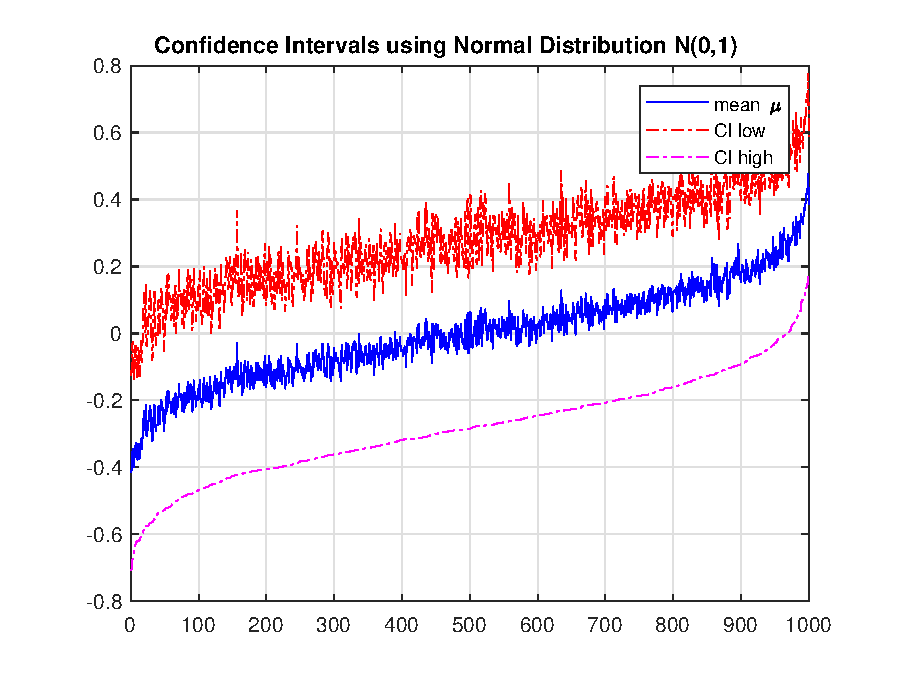
\includegraphics[width=\textwidth]{ex2_48_N}
		\caption{Results of the experiment with $n=48$ rvs $N(0,1)$}
		\label{fig:ex2_48_N}
	\end{minipage}
	\begin{minipage}{0.45\textwidth}
		\centering
		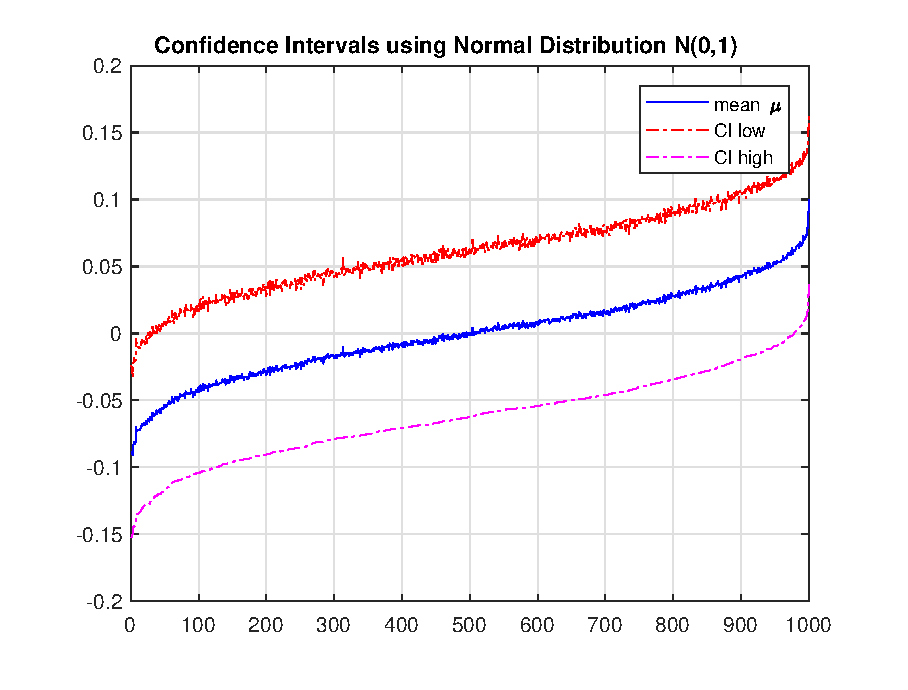
\includegraphics[width=\textwidth]{ex2_1000_N}
		\caption{Results of the experiment with $n=1000$ rvs $N(0,1)$}
		\label{fig:ex2_1000_N}
	\end{minipage}
\end{figure}

For the Exercise 4 the results are reported in \autoref{fig:ex4_N_accuracy} and \autoref{fig:ex4_N_CI}. As in exercise 4, is visible how, the accuracy get higher (that is, the distance between the sample mean and the true value get lower)  and the precision of the variance get higher (the \gls{ci} becomes smaller) as $n$ increases. Now the sample variance oscillates around $1$ that is in fact the new true value.

\begin{figure}[ht]
	\centering
	\begin{minipage}{0.45\textwidth}
		\centering
		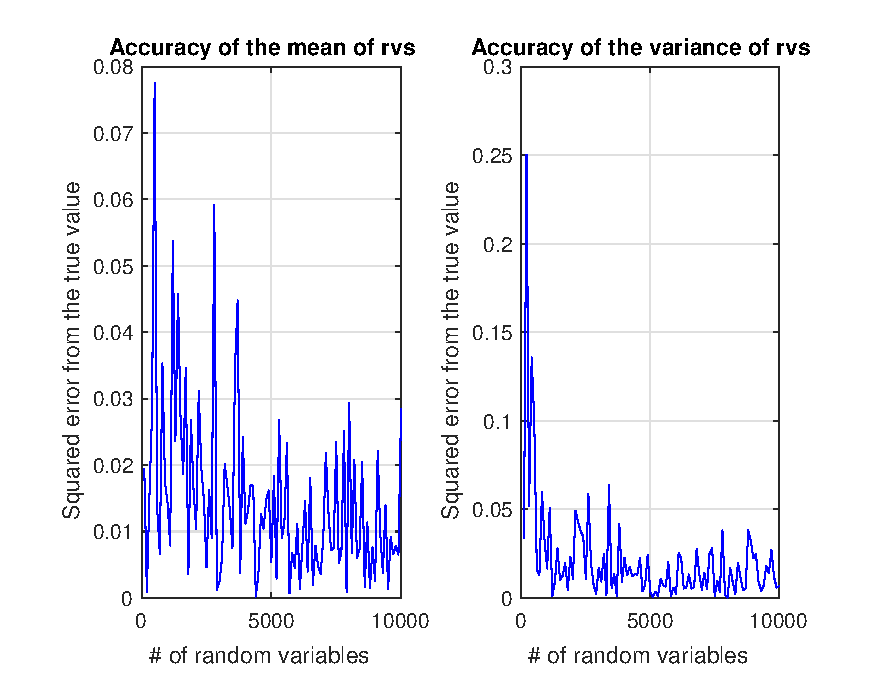
\includegraphics[width=\textwidth]{ex4_N_accuracy}
		\caption{Accuracy of the estimation versus $n$ using rvs $N(0,1)$}
		\label{fig:ex4_N_accuracy}
	\end{minipage}
	\begin{minipage}{0.45\textwidth}
		\centering
		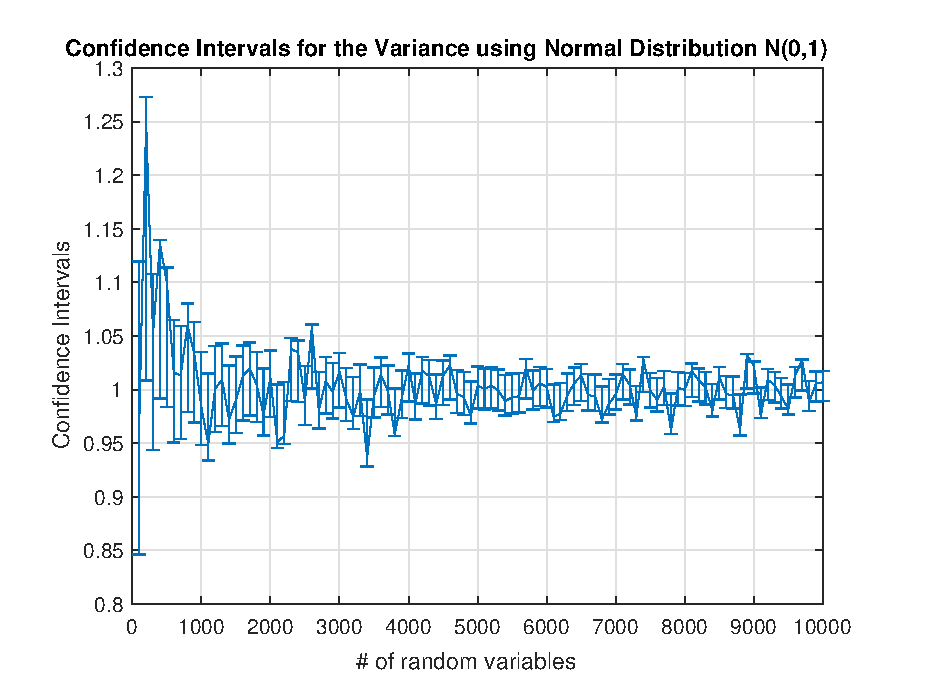
\includegraphics[width=\textwidth]{ex4_N_CI}
		\caption{Confidence intervals for the variance using rvs $N(0,1)$}
		\label{fig:ex4_N_CI}
	\end{minipage}
\end{figure}

For what regards the \gls{pi}, we can see that using the relative theory, the \gls{pi} is (as expected) between [-2,2], that is the $\gamma$ quantile of the Normal Distribution $N(0,1)$. In the bootstrap case, the result is very similar even if not so accurate as the theoretical result.

\begin{figure}[t]
	\centering
	\begin{minipage}{0.45\textwidth}
		\centering
		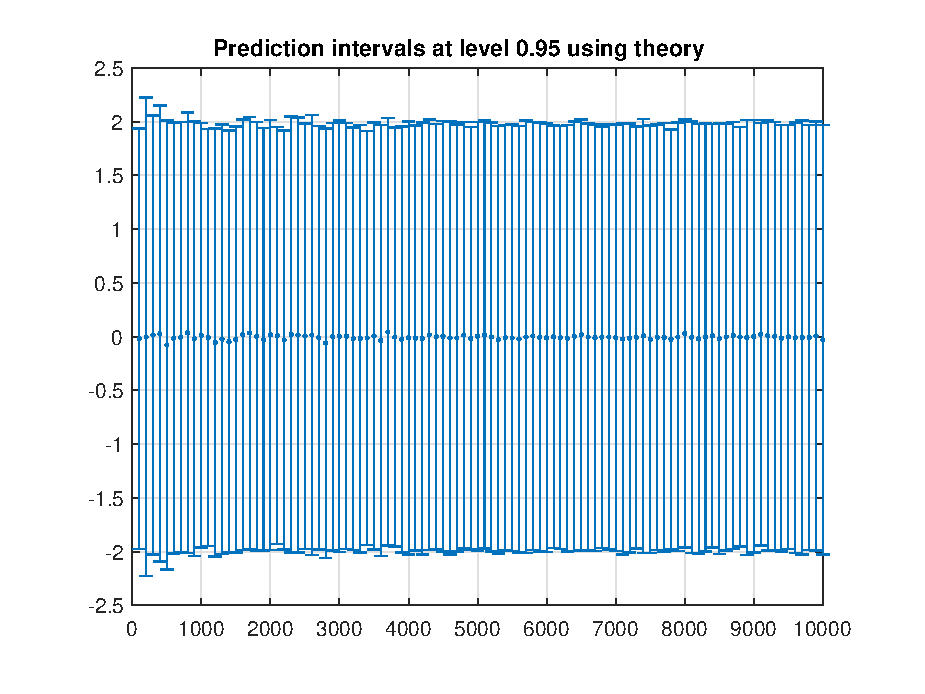
\includegraphics[width=\textwidth]{PI_theory_N}
		\caption{Prediction interval for a $N(0,1)$ at level $\gamma = 0.95$ using theory}
		\label{fig:PI_theory_N}
	\end{minipage}
	\begin{minipage}{0.45\textwidth}
		\centering
		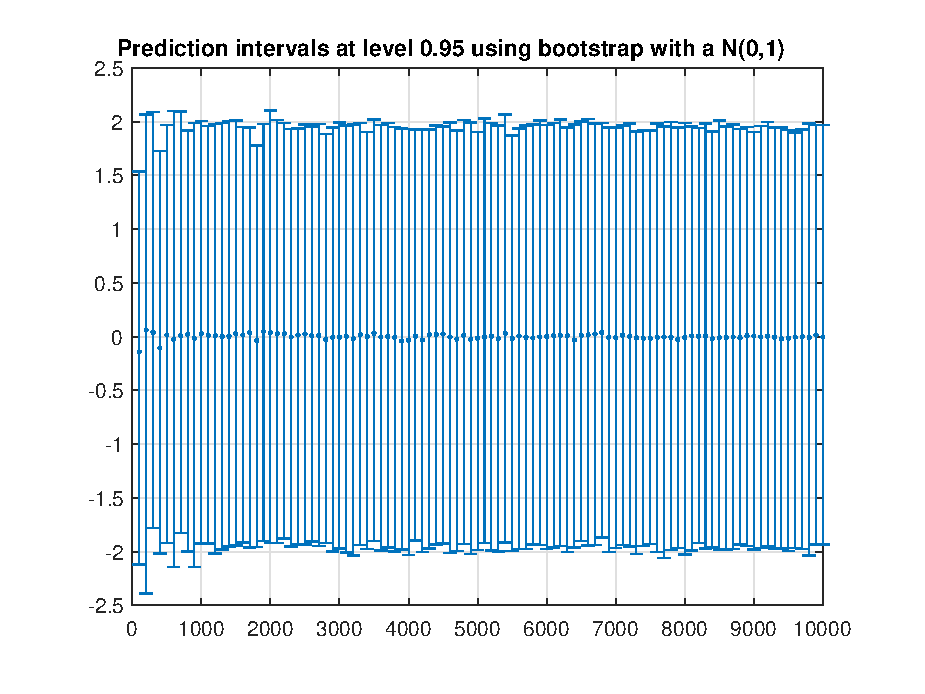
\includegraphics[width=\textwidth]{PI_bootstrap_N}
		\caption{Prediction interval for a $N(0,1)$ at level $\gamma = 0.95$ using bootstrap}
		\label{fig:PI_bootstrap_N}
	\end{minipage}
\end{figure}
\end{document}